\section{Problem Domain}

This chapter will analyze different aspects of the problem domain for our solution. The purpose of this is to produce a complete model of the problem domain, from which will answer the question: \textit{What data will the system process?}. 
We will accomplish this by looking at classes, structures and actions relevant to our system definition. \\
Our methods of analysis are borrowed from the book "Objected-oriented Design"\citep{FACTORPage}. It is recommended, although not necessary, to have knowledge of the methods used in the book. %In the following chapters we will refer to the program that we aim to make as our "solution".

The analysis of the problem domain consists of three points:
\begin{itemize}
\item \textbf{Classes:} Describes the system's classes.
\item \textbf{Events:} Lists events relating to the classes, resulting in a  
\item \textbf{Structure:} Describes the relationships between classes and objects, resulting in a class diagram.
\item \textbf{Behavior:} Describes the objects' behavior and interaction, and results in state diagrams.
\end{itemize}

By analyzing these different points of interest, insight is gained into which objects are relevant, what relations there are between them as well as their behavior.
With this insight it is easier to gauge how the system should be built, in order to handle the objects from the problem domain.

\subsection{Classes}

The problem domain can be described in terms of classes. Classes are the primary building blocks used to define and outline the problem domain. 

Through the process of brainstorming, we have been able to produce a list of classes that would be a good fit for the data that we would store.

The classes have been divided into four different groups, one group for each part of the program, as described in our system definition.

\subsubsection*{Main}
This is the main section of the program. When the user logs in to the program, they see information about their company. The main menu provides a variety of options, used to manage the company, and the projects it is currently working on. From this page it is also possible to view the company's employees and customers, along with additional information about them.

\begin{itemize}
  \item \textbf{Company} \\
 The company class is one of the main classes in the program. It will be used to keep track of the data of a specific company. A company can be created by a user and has users associated with it.
  
%This is the main module in the program. A company page is the hub for which all the information about the company is contained. It is possible to access multiple modules from this module. information such as VAT identification number (VATIN), clients and employees.
  
 % \item \textbf{Project Management} 
  
%When a company wants to produce something, or provide a service, they create a project for the company. This is done in the project management module. From here it is possible to assign employees to different projects, in different roles. From the project management page, you can choose from the different projects the company currently is working on, and view information about them. Each project has a separate budget, set by the project admin. This budget is used on salaries and product creation.
  
   information. 
  \item \textbf{User} \\
The user class identifies the users of the program. A user class can create or join companies, and its association with the company class, show its current status in a specific company, such as employer or employee.
  
%Contains information about the employees in a company. Information such as the employees names, rank and current projects.
\end{itemize}

\subsubsection*{CRM}

\begin{itemize}
  %\item \textbf{Documents} Information like document name, location, context etc.
  
  \item \textbf{Customer} \\
  The user class identifies the customers. It has attributes such as name, contact info. It is associated with the company class.
\end{itemize}

\subsubsection*{Project}

\begin{itemize}
  \item \textbf{Project} \\
This class contains information about projects, with attributes such as project name and users connected to the project. It is associated with both the user, company and customer classes.
  \item \textbf{Task} \\
Information about tasks that are connected to individual projects. Attributes such as name, description, employee(s) assigned, deadline.
  \item \textbf{Task Comment} \\
Users can comment on an existing task. that are connected to individual projects. Attributes like comment content and employee.

\end{itemize}



\subsubsection*{Finance}

\begin{itemize}
  \item \textbf{Budget} \\
  This class contains finance information, such as expenditure and income. 
  % Taxes, capital, profit reinvestment.
 
  %\item \textbf{Income} Information such as, name, company, time etc.

\end{itemize}

\subsection{Events}
From the classes, we have below derived a number of events that could take place between objects from the different classes. Identifying these events is important, as it improves our knowledge of what needs to be implemented in the program.

To create an overview of the events and the connection between events and classes, we have created an event table. By looking at the event table you can quickly see what events are related to which classes.
That there is a symbol indicates, a relation between an event and a class. The "+" symbol indicates that the event can happen 0 and 1 times for each object and the "*" symbol indicates that the event can happen 0 or more times.


\hspace*{-2,5cm}
\begin{tabular}{|l||c|c|c|c|c|c|c|c|}
  \hline
                                   & Company & Employee & Project & Customer & Budget  & Product & Task    & TC*             \\\hline \hline
   Customer added                  &    *    &          &         &     +    &         &         &         &                 \\\hline
   Customer updated                &    *    &          &         &     *    &         &         &         &                 \\\hline 
   Customer deleted                &    *    &          &         &     +    &         &         &         &                 \\\hline
   Project added                   &    *    &    *     &    +    &     *    &         &         &         &                 \\\hline
   Project updated                 &         &    *     &    *    &          &         &         &         &                 \\\hline
   Project deleted                 &    *    &    *     &    +    &     *    &         &         &         &                 \\\hline
   Task added                      &         &          &    +    &          &         &         &   +     &   *             \\\hline 
   Task deleted                    &         &          &    *    &          &         &         &   +     &   +             \\\hline
   Task updated                    &         &    *     &    *    &          &         &         &   *     &   *             \\\hline
   Task finished                   &         &    *     &    *    &          &         &         &   +     &   +             \\\hline
   TC added                        &         &    *     &         &          &         &         &   *     &   *             \\\hline
   TC updated                      &         &    *     &         &          &         &         &   *     &   *             \\\hline
   TC deleted                      &         &    *     &         &          &         &         &   *     &   *             \\\hline
   Product added                   &    *    &          &         &          &         &    +    &         &                 \\\hline
   Product deleted                 &    *    &          &         &          &         &    +    &         &                 \\\hline
   Product updated                 &    *    &          &         &          &         &    *    &         &                 \\\hline
   Income added                    &    *    &          &         &     *    &    +    &         &         &                 \\\hline
   Income updated                  &    *    &          &         &     *    &    *    &         &         &                 \\\hline
   Expense added                   &    *    &          &         &     *    &    +    &    *    &         &                 \\\hline
   Expense updated                 &    *    &          &         &     *    &    *    &         &         &                 \\\hline
   Employee added                  &    *    &    +     &         &          &         &         &         &                 \\\hline
   Employee updated                &    *    &    *     &         &          &         &         &         &                 \\\hline
   Company added                   &    +    &          &         &          &         &         &         &                 \\\hline
   Company updated                 &    *    &          &         &          &         &         &         &                 \\
  \hline
\end{tabular}
\textit{* TC stands for Task Comment}
                                                                                                                                 
Based on the event table, each class has an adequate amount of events attached. Since the events are spread out over the classes, it means that there is no one class that has too many events compared to the other classes. %Had there been a class with too many events, we should have considered if it could be divided into several classes. 

\subsection{Structure}
To describe the relations between the different classes, a class diagram has been created.

\begin{figure}[H]
    \centering
    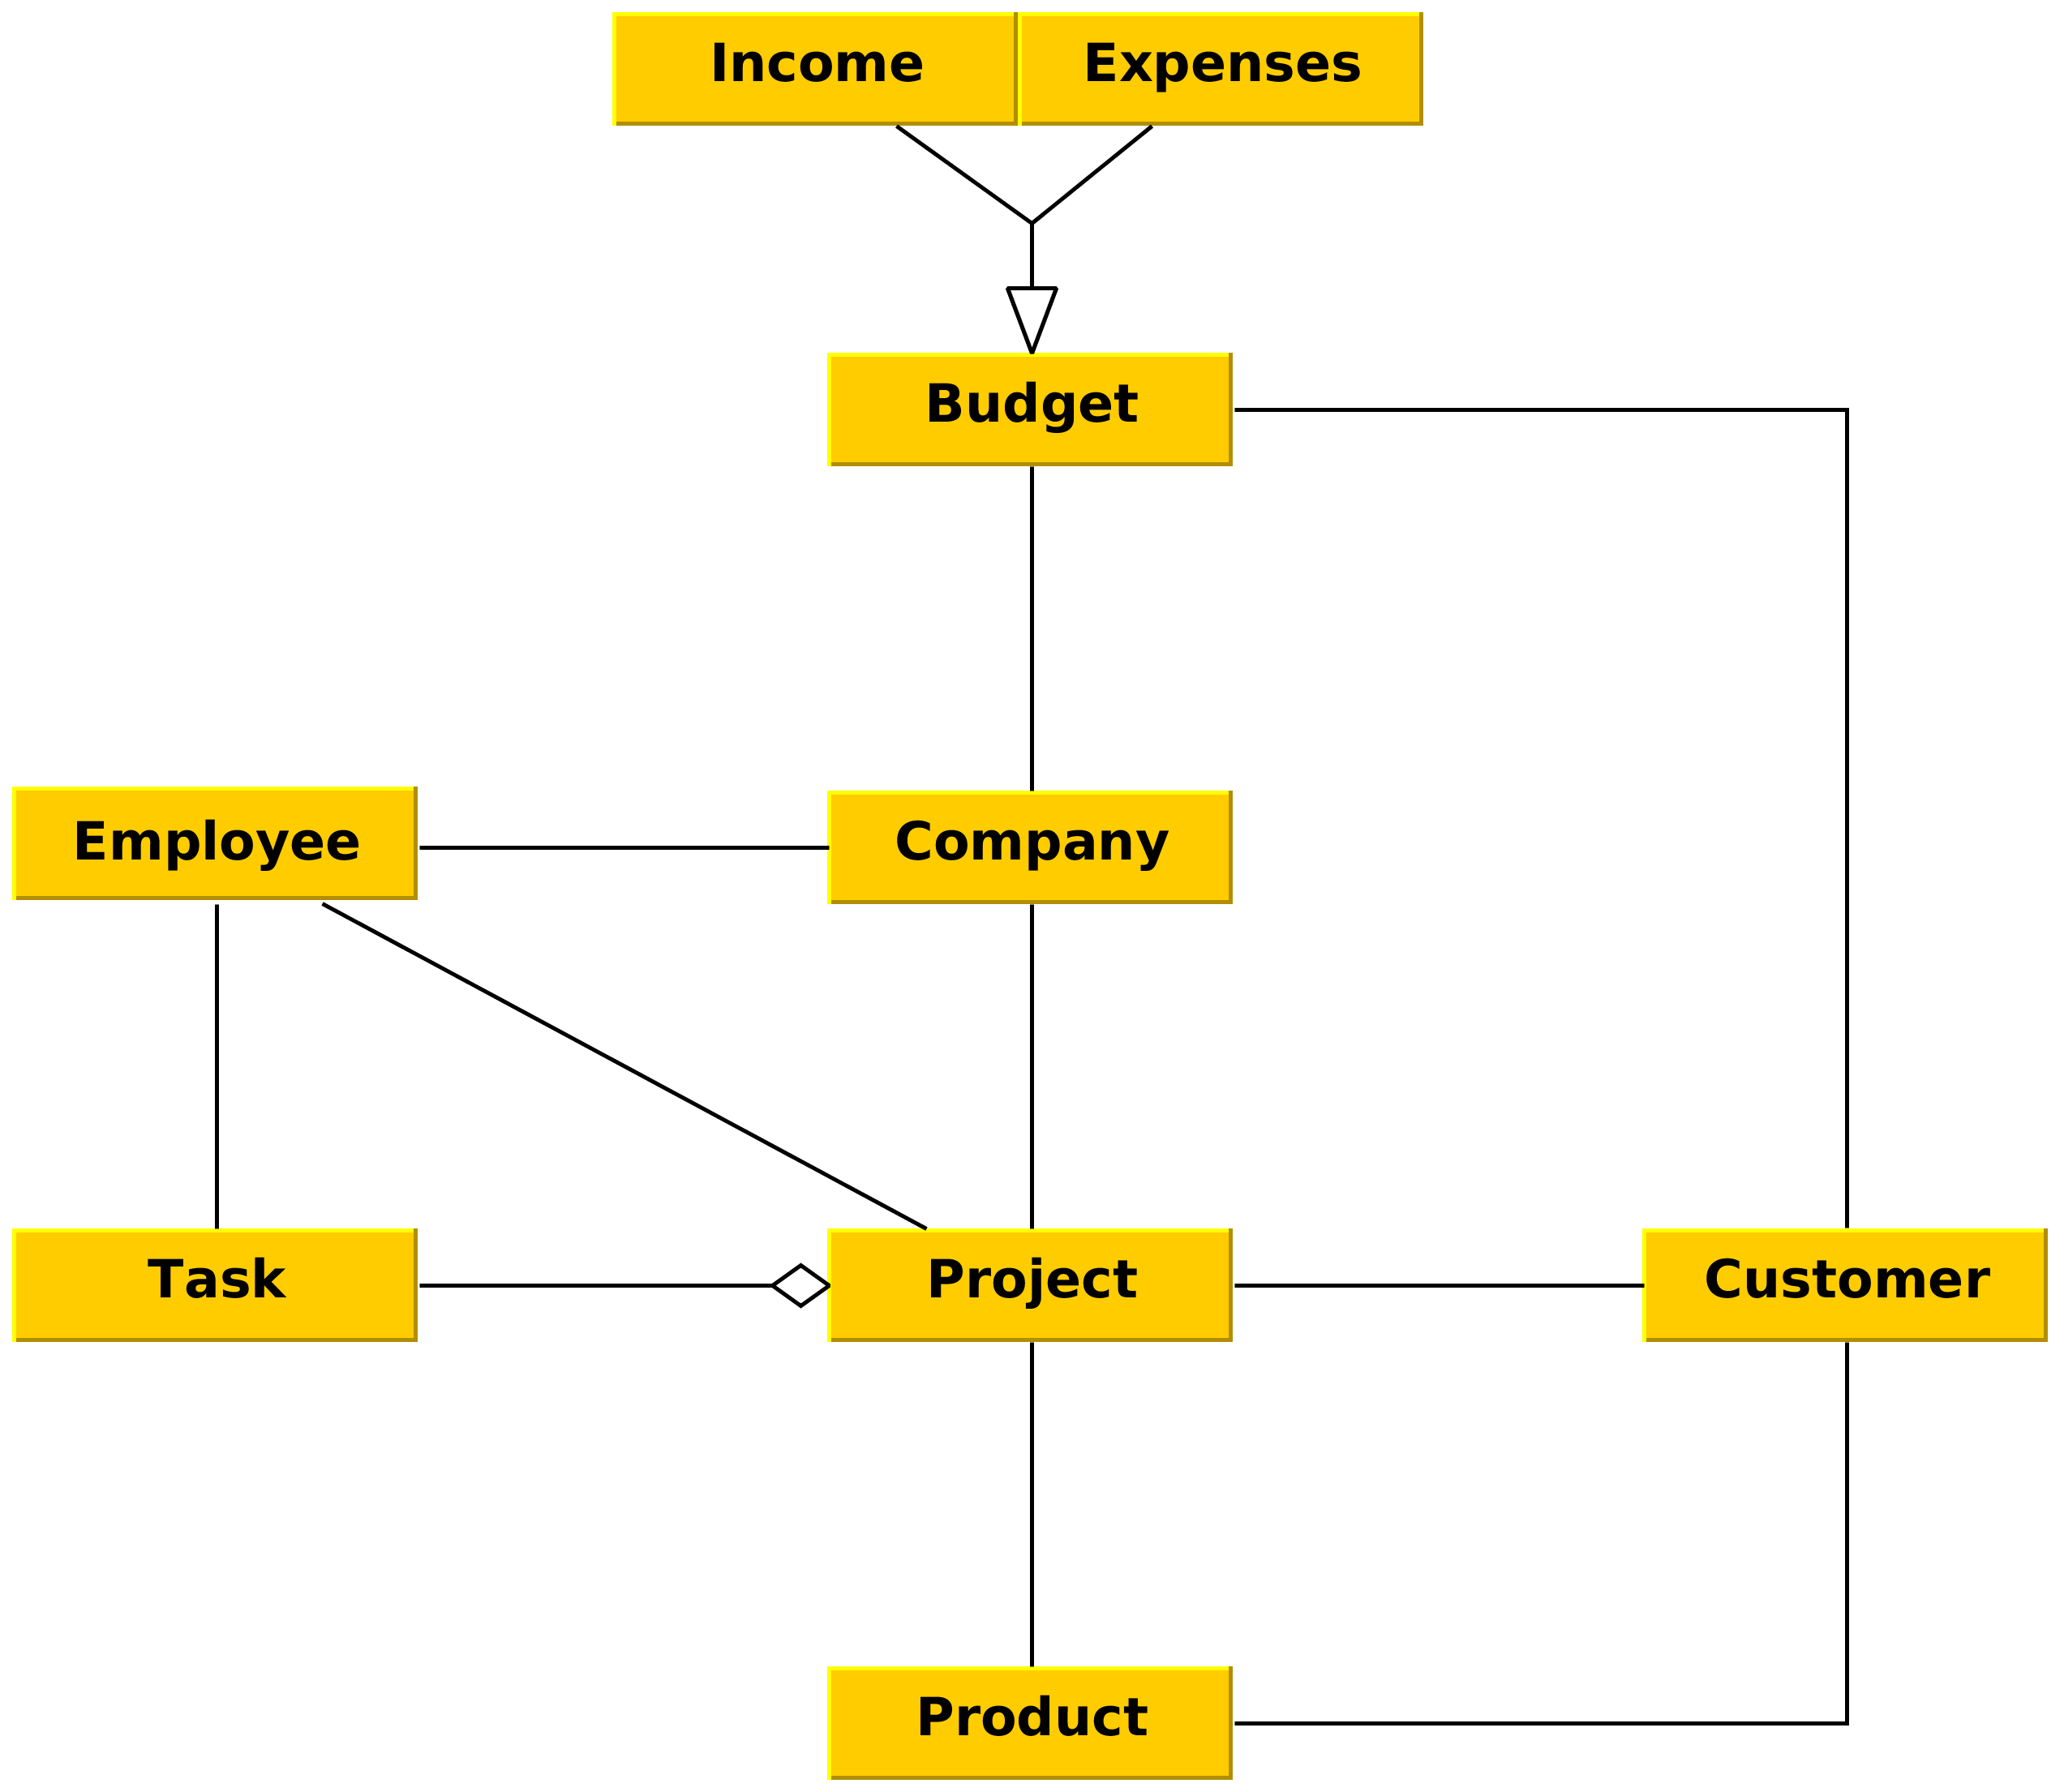
\includegraphics[scale=0.12]{Images/ProblemDomain/klassediagram.png}
    \caption{Class Diagram ???????}
    \label{fig:Class Diagram}
\end{figure}

\subsection{Behavior}

Based on the events in the event table, we can make behavioral patterns. The overall behavior of different objects is made up of the order in which events are run (event traces) and the behavioral patterns of the given object. %An event trace, a sequence of events, describes in which order different events can be run for a given object. 
\\
Behavioral patterns can be described by statechart diagrams. State diagrams give an abstract description of system behavior, by taking an object of a single class and showing the different states it will inhabit as it goes through the system.
We have therefore made statechart diagrams of some of the more important events. These statechart diagrams will be based on the events we uncovered in the event table.



\subsubsection*{Company}

\begin{figure}[H]
    \centering
    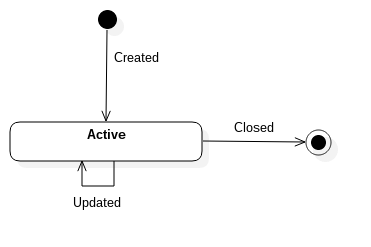
\includegraphics[scale=0.7]{Images/ProblemDomain/companyActivityDiagram.png}
    \caption{Company Activity}
    \label{fig:companyActivityDiagram}
\end{figure}

The company is a shitty class that shits all over your face, so prepare yourself and by that i mean your face. Your face will be in big pain because the shit contains a lot of chili so it will burn especially in your eyes. BTW we of the PYFFS(Protect Your Face From Shit) association recommend closing your eyes when it happens. If you don't close your eyes, there is 60\%+ chance of getting blind. other than that you will only lose about 80\% feeling in your face because of the chili from the shit that will hit your face very hard. \\
If you have just read the following line, it means you have passed the test of reading the rapport :) High-Five for u!


\subsubsection*{Customer}

\begin{figure}[H]
    \centering
    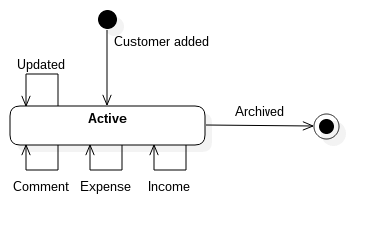
\includegraphics[scale=0.7]{Images/ProblemDomain/customerActivityDiagram.png}
    \caption{Customer Activity}
    \label{fig:customerActivityDiagram}
\end{figure}

\subsubsection*{Employee}

\begin{figure}[H]
    \centering
    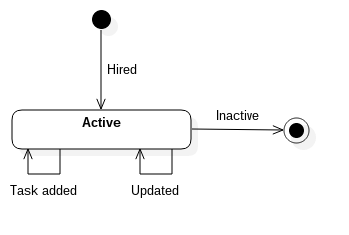
\includegraphics[scale=0.7]{Images/ProblemDomain/employeeActivityDiagram.png}
    \caption{Employee Activity}
    \label{fig:employeeActivityDiagram}
\end{figure}

\subsubsection*{Project}

\begin{figure}[H]
    \centering
    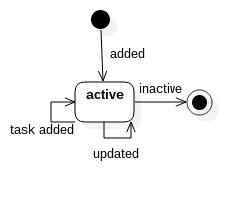
\includegraphics[scale=0.7]{Images/ProblemDomain/projectActivityDiagram.png}
    \caption{Project Activity}
    \label{fig:projectActivityDiagram}
\end{figure}

\subsubsection*{Product}

\begin{figure}[H]
    \centering
    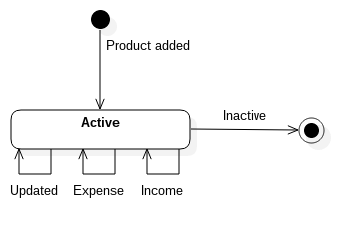
\includegraphics[scale=0.7]{Images/ProblemDomain/productActivityDiagram.png}
    \caption{Project Acitivty}
    \label{fig:productAcitvityDiagram}
\end{figure}

\subsubsection*{Task}

\begin{figure}[H]
    \centering
    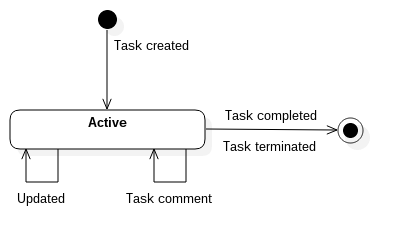
\includegraphics[scale=0.7]{Images/ProblemDomain/taskActivityDiagram.png}
    \caption{Task Activity}
    \label{fig:taskActivityDiagram}
\end{figure}

\subsubsection*{Task comment}

\begin{figure}[H]
    \centering
    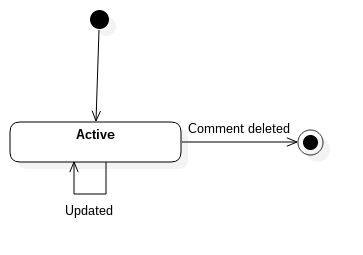
\includegraphics[scale=0.7]{Images/ProblemDomain/tcActivityDiagram.png}
    \caption{Task comment Activity}
    \label{fig:tcActivityDiagram}
\end{figure}

\subsubsection*{Budget}

\begin{figure}[H]
    \centering
    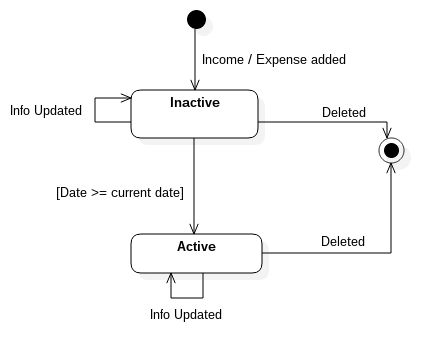
\includegraphics[scale=0.7]{Images/ProblemDomain/budgetActivityDiagram.png}
    \caption{Budget Activity}
    \label{fig:budgetActivityDiagram}
\end{figure}
















\subsection{Summary}

In this chapter the different classes relevant to the problem domain have been found. Events have been found for each of these classes. 
Based on those events a class diagram has been produced, demonstrating the relations between the different classes. Furthermore the behavior of a number of important classes has been analyzed. Based on all this is now a foundation for what classes the final program should contain, their relations and their behavior.

The next chapter will focus on the context in which the solution would be used. The chapter take a closer look at what the solution should be able to do, how users will be using the solution and to best make the solution fit the needs of the users.














